\documentclass[paper=letter,11pt]{scrartcl}

\KOMAoptions{headinclude=true, footinclude=false}
\KOMAoptions{DIV=14, BCOR=5mm}
\KOMAoptions{numbers=noendperiod}
\KOMAoptions{parskip=half}
\addtokomafont{disposition}{\rmfamily}
\addtokomafont{part}{\LARGE}
\addtokomafont{descriptionlabel}{\rmfamily}
%\setkomafont{pageheadfoot}{\normalsize\sffamily}
\setkomafont{pagehead}{\normalsize\rmfamily}
%\setkomafont{publishers}{\normalsize\rmfamily}
\setkomafont{caption}{\normalfont\small}
\setcapindent{0pt}
\deffootnote[1em]{1em}{1em}{\textsuperscript{\thefootnotemark}\ }


\usepackage{amsmath}
\usepackage[varg]{txfonts}
\usepackage[T1]{fontenc}
\usepackage{graphicx}
\usepackage{xcolor}
\usepackage[american]{babel}
% hyperref is needed in many places, so include it here
\usepackage{hyperref}

\usepackage{xspace}
\usepackage{multirow}
\usepackage{float}


\usepackage{braket}
\usepackage{bbm}
\usepackage{relsize}
\usepackage{tcolorbox}

\def\ketY{\ensuremath{\ket {\Psi}}}
\def\iGeV{\ensuremath{\textrm{GeV}^{-1}}}
%\def\mp{\ensuremath{m_{\textrm{proton}}}}
\def\rp{\ensuremath{r_{\textrm{proton}}}}
\def\me{\ensuremath{m_{\textrm{electron}}}}
\def\aG{\ensuremath{\alpha_G}}
\def\rAtom{\ensuremath{r_{\textrm{atom}}}}
\def\rNucl{\ensuremath{r_{\textrm{nucleus}}}}
\def\GN{\ensuremath{\textrm{G}_\textrm{N}}}
\def\ketX{\ensuremath{\ket{\vec{x}}}}
\def\ve{\ensuremath{\vec{\epsilon}}}


\def\ABCDMatrix{\ensuremath{\begin{pmatrix} A &  B  \\ C  & D \end{pmatrix}}}
\def\xyprime{\ensuremath{\begin{pmatrix} x' \\ y' \end{pmatrix}}}
\def\xyprimeT{\ensuremath{\begin{pmatrix} x' &  y' \end{pmatrix}}}
\def\xy{\ensuremath{\begin{pmatrix} x \\ y \end{pmatrix}}}
\def\xyT{\ensuremath{\begin{pmatrix} x & y \end{pmatrix}}}

\def\IMatrix{\ensuremath{\begin{pmatrix} 0 &  1  \\ -1  & 0 \end{pmatrix}}}
\def\IBoostMatrix{\ensuremath{\begin{pmatrix} 0 &  1  \\ 1  & 0 \end{pmatrix}}}
\def\JThree{\ensuremath{\begin{pmatrix}    0 & -i & 0  \\ i & 0  & 0 \\ 0 & 0 & 0 \end{pmatrix}}} 
\def\JTwo{\ensuremath{\begin{bmatrix}    0 & 0 & -i  \\ 0 & 0  & 0 \\ i & 0 & 0 \end{bmatrix}}}
\def\JOne{\ensuremath{\begin{bmatrix}    0 & 0 & 0  \\ 0 & 0  & -i \\ 0 & i & 0 \end{bmatrix}}}
\def\etamn{\ensuremath{\eta_{\mu\nu}}}
\def\Lmn{\ensuremath{\Lambda^\mu_\nu}}
\def\dmn{\ensuremath{\delta^\mu_\nu}}
\def\wmn{\ensuremath{\omega^\mu_\nu}}
\def\be{\begin{equation*}}
\def\ee{\end{equation*}}
\def\bea{\begin{eqnarray*}}
\def\eea{\end{eqnarray*}}
\def\bi{\begin{itemize}}
\def\ei{\end{itemize}}
\def\fmn{\ensuremath{F_{\mu\nu}}}
\def\fMN{\ensuremath{F^{\mu\nu}}}
\def\bc{\begin{center}}
\def\ec{\end{center}}
\def\nus{$\nu$s}

\def\adagger{\ensuremath{a_{p\sigma}^\dagger}}
\def\lineacross{\noindent\rule{\textwidth}{1pt}}

\newcommand{\multiline}[1] {
\begin{tabular} {|l}
#1
\end{tabular}
}

\newcommand{\multilineNoLine}[1] {
\begin{tabular} {l}
#1
\end{tabular}
}



\newcommand{\lineTwo}[2] {
\begin{tabular} {|l}
#1 \\
#2
\end{tabular}
}

\newcommand{\rmt}[1] {
\textrm{#1}
}


%
% Units
%
\def\m{\ensuremath{\rmt{m}}}
\def\GeV{\ensuremath{\rmt{GeV}}}
\def\pt{\ensuremath{p_\rmt{T}}}


\def\parity{\ensuremath{\mathcal{P}}}

\usepackage{cancel}
\usepackage{ mathrsfs }
\def\bigL{\ensuremath{\mathscr{L}}}

\usepackage{ dsfont }



\usepackage{fancyhdr}
\fancyhf{}


\lhead{\Large 33-444} % \hfill Introduction to Particle Physics \hfill Spring 2022}
\chead{\Large Introduction to Particle Physics} % \hfill Spring 2022}
\rhead{\Large Spring 2022} % \hfill Introduction to Particle Physics \hfill Spring 2022}
\begin{document}
\thispagestyle{fancy}


\begin{center}
{\huge \textbf{Homework Set \#9 }}
\large


\end{center}

{\large


\textbf{4)  $W$ boson decays to electrons. } \hfill \textit{(3 points)}\\
\begin{itemize}
\item[a)]{ The W can decay directly to an electron or to electron by decaying through a $\tau$. Draw the corresponding diagrams.
\bc
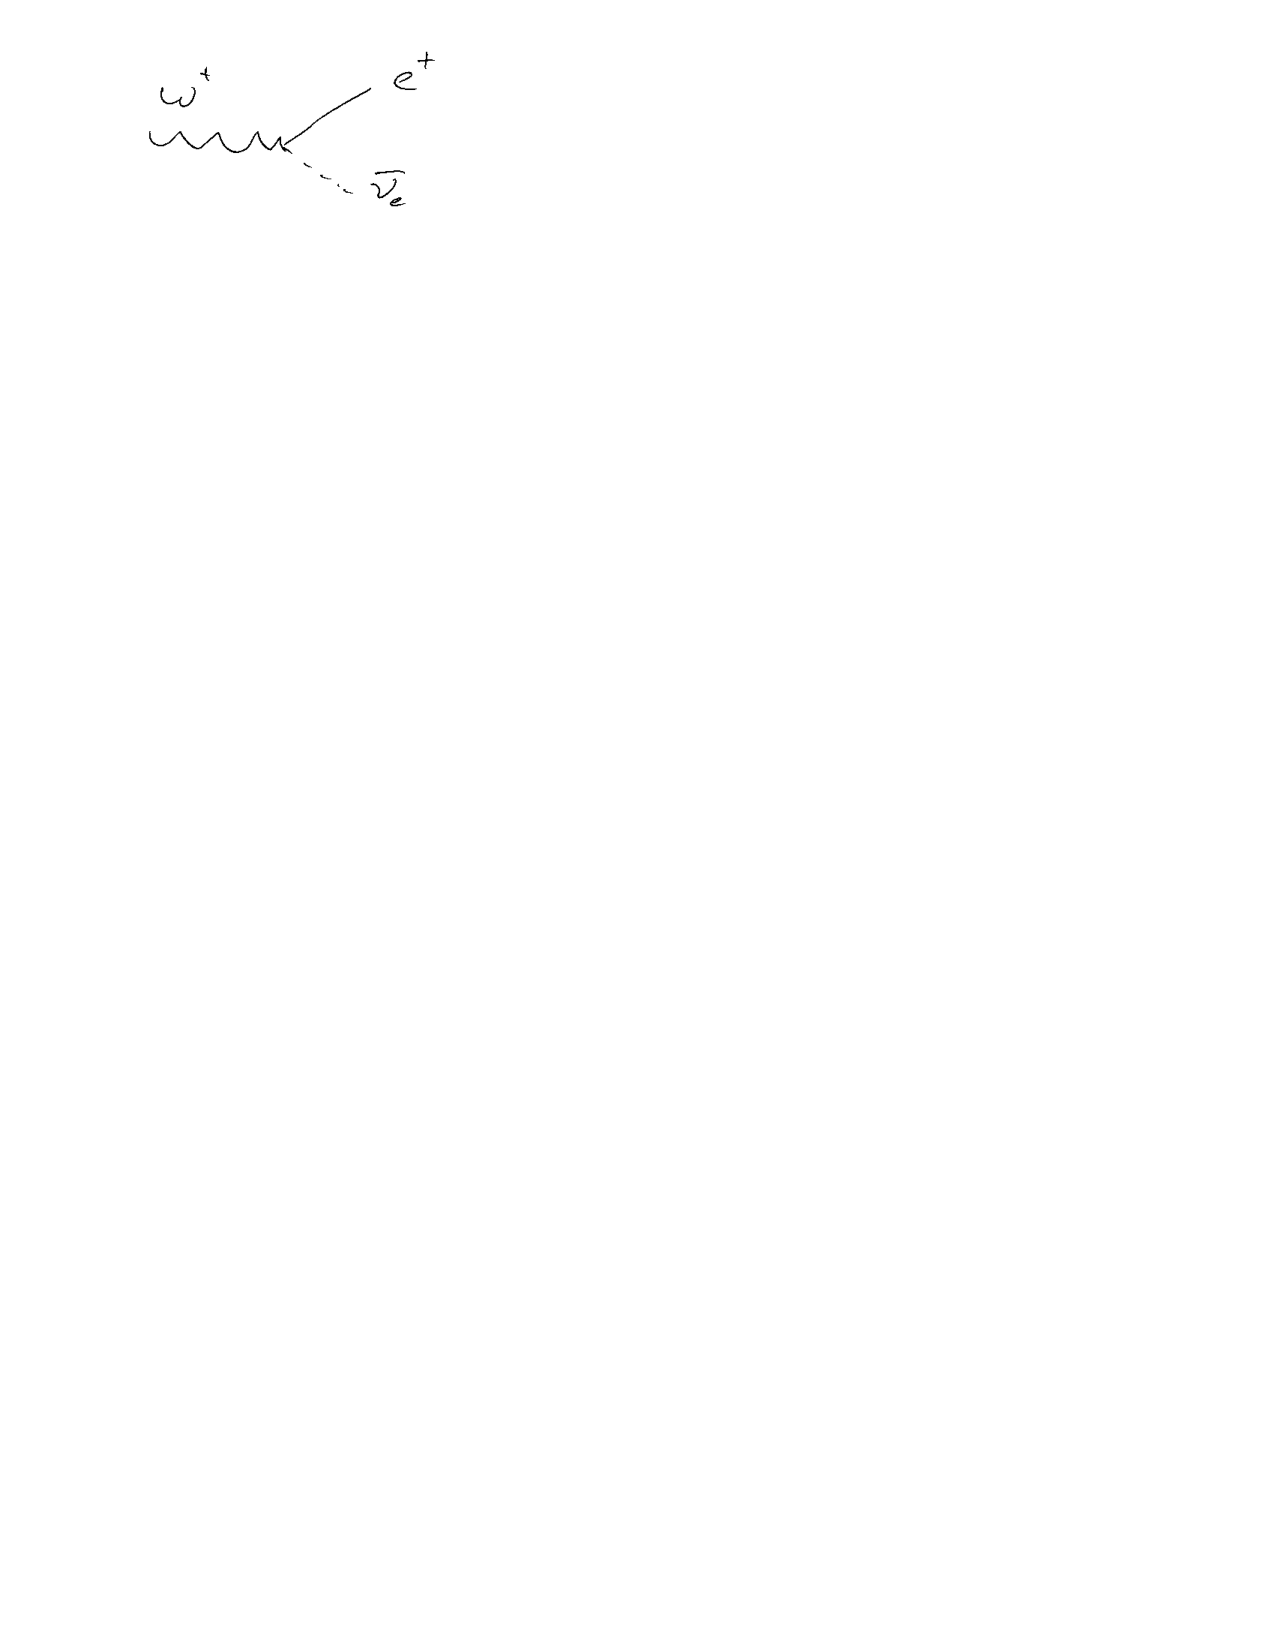
\includegraphics[width=0.3\textwidth]{./Wenu.pdf}
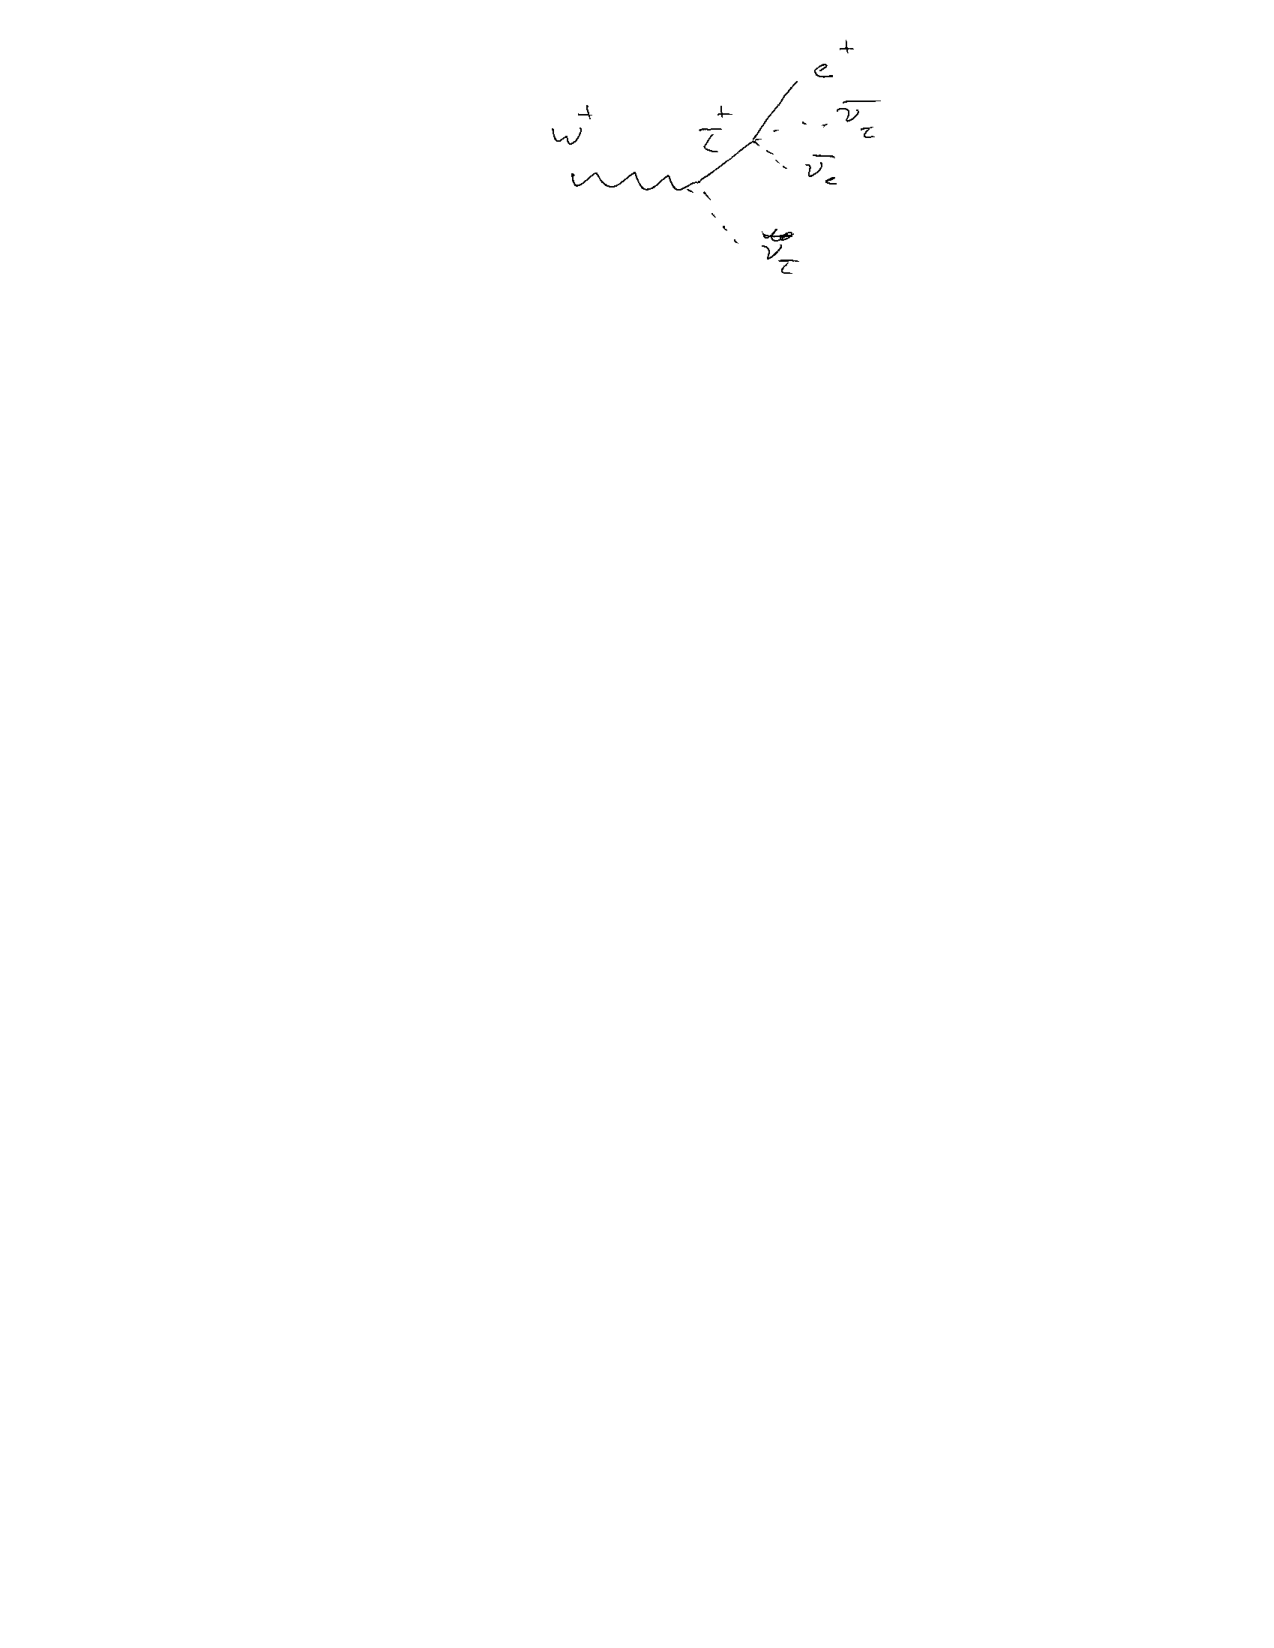
\includegraphics[width=0.3\textwidth]{./We3nu.pdf}
\ec
}
\item[b)]{ 
\be
Br(W\rightarrow \ell \nu)  = \frac{1}{\underbrace{3}_{\rmt{leptons}} + \underbrace{3}_{\rmt{color}} \times \underbrace{2}_{\rmt{2 quark generations}}} = \frac{1}{9} = 0.11
\ee
(Note the top-quark is heavier than the W, so the $W\rightarrow t, b $ decay is forbidden.)

Now,
\be
Br(\tau \rightarrow e \nu \bar{\nu})  = \frac{1}{\underbrace{2}_{\rmt{leptons}} + \underbrace{3}_{\rmt{color}} \times \underbrace{2}_{\rmt{1 quark generations}}} = \frac{1}{5} = 0.2
\ee
Here the $\tau$ can decay to two lepton generation (es and $\mu$ s), but only has enough mass to decay to one quark generation (u, d). 


So, 
\be
Br(W\rightarrow e + X) = \underbrace{\frac{1}{9}}_{W\rightarrow e\nu} + \underbrace{\frac{1}{9}}_{W\rightarrow \tau\nu} \times \underbrace{\frac{1}{5}}_{\tau\rightarrow e\nu}  = \frac{1.2}{9} = 0.13
\ee

}
\end{itemize}           

\textbf{4) $ H\rightarrow WW\rightarrow e \mu$ decaus. } \hfill \textit{(3 points)}\\

\be
Br(W\rightarrow \ell \nu) \sim \frac{1}{9} 
\ee

for e or $\mu$ can include the decays through $\tau$s as in problem 3 to get $\frac{1.2}{9}$

\be
Br(WW\rightarrow e\mu + X) = 2 \times \left(\frac{1.2}{9}\right)^2 \sim 0.036
\ee
Factor of two becuase you can get $e^+\mu^-$ or $e^-\mu^+$



\textbf{2) Tracking Detectors } \hfill \textit{(10 points)}\\
\begin{itemize}
\item[a)]{
\be
F = ma \Rightarrow m v^2/r_c = qvB  \Rightarrow r_c = p_T/qB
\ee
Now,
\be
r_c^2 = \left(\frac{L}{2}\right)^2 + (r_c -s )^2
\ee
Or (Ignoring terms 
\be
\frac{L^2}{4} = 2 r_c s - s^2
\ee
B/c $r_c >> s$, can safely drop $s^2$ relative to $r_c s$.  Thus
\be
s = \frac{L^2}{8r_c} = \frac{qBL^2}{8p_T}
\ee


}
\item[b)]{
\be
p_T = \frac{qBL^2}{8s}
\ee 
So,
\be
\Delta p_T = \frac{qBL^2}{8s^2} \Delta s 
\ee 

and
\be
\frac{\Delta p_T}{p_T} = \frac{\Delta s}{s} = \frac{8p_T}{qBL^2} \Delta s 
\ee 

}
\item[c)]{
For N = 50, $\epsilon$ = 100 $\mu m$, L = 1 m, and B = 1 T, $\Delta s \sim 50 \mu m = 50 10^{-6} m$

Now
$T = 2 \times 10^{-16} GeV^2$\\
$e = 0.3$
\be
\Delta p_T = \frac{8 (p_T[GeV])^2}{0.3 \times 2 \times 10^{-16} }  \frac{50 \times 10^{-6}}{5\times10 ^{15} GeV^{-1}} \sim 3\times10^{-3} (p_T[GeV])^2 GeV
\ee

At 1 GeV the uncertainty is $\sim 10^{-3}$ GeV,   At 100 GeV the uncertainty is 10 GeV.
}
\end{itemize}

\clearpage


\textbf{3) Limits of the Tracking System.} \hfill \textit{(5 points)}\\

\begin{itemize}
\item[a)]{
\be
r_c \sim 3 \frac{p_T[GeV] }{Q[e] B[T]}
\ee
Particles dont make it to the calorimeter when $r_{calo} \sim 2\times r_c$

or 
\be
p_T \sim \frac{q B r_{calo}}{6} = \frac{2 \times 1.1}{6} \sim 400 MeV
\ee

}

\item[b)]{
Estimate upper limit when $s\sim17 \mu m \sim 20 \times 10^{-6} m$

\be
p_T \sim \frac{0.3 \times 2\times 10^{-16} GeV^2}{8} \frac{0.5}{20 \times 10^{-6}} 0.5 \times 5 \times 10^{15} GeV^{-1}
p_T \sim 0.5\times 10^3 GeV
\ee

}
\item[c)]{
At the limit $\Delta s / s \sim 1  \Rightarrow \Delta p_T / p_T \sim 1 $, so $\Delta p_T \sim 500$ GeV


}
\end{itemize}

\vspace*{0.25in}

\textbf{4) Rapidity.} \hfill \textit{(15 points)}\\

\begin{itemize}
\item[a)]{
Under a boost along Z

\be
E \rightarrow E \gamma - \beta \gamma p_z
\ee
\be
p_z \rightarrow p_z \gamma - \beta \gamma E
\ee

So,

\begin{align*}
y \rightarrow \frac{1}{2} \log \frac{(E \gamma - \beta \gamma p_z) + (p_z \gamma - \beta \gamma E)}{(E \gamma - \beta \gamma p_z) -(p_z \gamma - \beta \gamma E)} \\ 
  = \frac{1}{2} \log \frac{\gamma - \beta \gamma}{\gamma + \beta \gamma}\frac{E+p_z}{E - p_z} = \frac{1}{2} \log \frac{E+p_z}{E - p_z} + \frac{1}{2} \log \frac{\gamma - \beta \gamma}{\gamma + \beta \gamma}\\
  = y + \frac{1}{2} \log \frac{\cosh \eta - \sinh \eta}{\cosh + \sinh \eta} = y + \frac{1}{2} \log \frac{e^{-\eta}} {e^{+\eta}}\\
  = y + \frac{1}{2} \log e^{-2\eta} = y - \eta
 \end{align*}

}
\item[b.]{
$y = \eta $ for mass-less particles
}
\item[d.]{
Green are electrons / Red are muons.
}
\item[e]{
I got:

eta1 = -1  /
phi1 = 70 /
pt1  = 30 

eta2 = 0  /
phi2 = 255 /
pt2  = 30 

eta3 = -0.2 / 
phi3 = 70  /
pt3  = 20

eta4 = 0.5 / 
phi4 = 200 /
pt4  = 25 

}
\item[f.]{
I get: (124.8, -14.2, 9.5, -26.3) GeV (E,vec{P})
}
\item[h.]{68. probably Zboson}
\item[i.]{43 probably off shell z}
\item[j.]{121 GeV probably a higgs}





\end{itemize}




}
\end{document}
